\chapter{Fundamentação Teórica}
\label{cap:fundamentacao-teorica}

Neste capítulo são apresentados os conceitos usados ao longo deste trabalho. Primeiro, é feita uma explicação sobre a retina, o exame de fundoscopia e a retinopatia diabética, com foco nos exsudatos duros e moles. Em seguida, apresentam-se o pré-processamento das imagens, os fundamentos de aprendizado profundo e as redes que serão comparadas, e por último a segmentação, as funções de perda, a validação, as métricas, os testes estatísticos e os sistemas de diagnóstico auxiliado por computador (CAD, do inglês \textit{Computer-Aided Diagnosis}).

\section{Anatomia da retina e fundoscopia}
\label{sec:anatomia-retina}

A retina é a camada mais interna do olho, onde a luz focalizada pela córnea e pelo cristalino é convertida em sinais nervosos pelos fotorreceptores (cones e bastonetes). Esses sinais seguem pelas fibras nervosas até o disco óptico e, pelo nervo óptico, chegam ao cérebro \cite{abramoff2010retinal}.

Algumas estruturas aparecem com frequência na análise das imagens. O disco óptico é a região por onde saem as fibras do nervo óptico e por onde passam os vasos da retina, e aparece nas imagens como uma área arredondada e clara. A mácula fica perto do centro da retina e, no seu centro, está a fóvea, com grande concentração de cones e responsável pela visão central e detalhada \cite{abramoff2010retinal}, por isso lesões próximas da fóvea tendem a afetar mais a visão. Os vasos partem do disco óptico e se ramificam pela retina, e são os pequenos vasos e capilares que a retinopatia diabética afeta primeiro \cite{cheung2010dr}.

A fundoscopia, ou oftalmoscopia, é o exame que permite observar o fundo do olho através da pupila. Quando essa observação é registrada por uma câmera de fundo de olho, o resultado é uma fotografia colorida da retina, chamada de retinografia \cite{abramoff2010retinal}. As imagens da base IDRiD (\textit{Indian Diabetic Retinopathy Image Dataset}), por exemplo, foram obtidas com uma câmera Kowa VX-10$\alpha$, com campo de visão de 50 graus e resolução de $4288 \times 2848$ pixels \cite{porwal2018idrid}.

A retinografia é muito usada no rastreamento da retinopatia diabética, por ser rápida e não invasiva, e as imagens podem ser enviadas e analisadas à distância, no que se chama de telerrastreamento \cite{abramoff2010retinal}. Contudo, as imagens variam bastante entre locais de aquisição, em função da câmera, da iluminação, do foco e da dilatação da pupila \cite{abramoff2010retinal}. Por esse motivo, um modelo com bom desempenho em uma base pode apresentar resultados piores em outra.

\section{Retinopatia diabética}
\label{sec:retinopatia}

A retinopatia diabética (RD) é uma complicação microvascular do diabetes mellitus. A hiperglicemia mantida por muito tempo danifica os pequenos vasos da retina, com perda de pericitos e quebra da barreira hematorretiniana, de modo que os vasos passam a deixar escapar sangue, líquido e lipídios e, em fases mais avançadas, alguns capilares se fecham, causando falta de oxigenação (isquemia) \cite{cheung2010dr}. Nas fases iniciais, a doença costuma ser assintomática, e o paciente pode perceber a perda de visão apenas quando o quadro já está avançado \cite{brasil2021pcdtrd}.

A RD é dividida em duas fases. Na forma não proliferativa (RDNP) aparecem microaneurismas, hemorragias, exsudatos e alterações venosas, e na forma proliferativa (RDP) a isquemia estimula o crescimento de vasos novos e frágeis (neovascularização), que podem sangrar. Em qualquer fase pode ocorrer o edema macular diabético, que é o acúmulo de líquido na mácula e uma das principais causas de perda de visão em pessoas com diabetes \cite{cheung2010dr}.

\subsection{Lesões da retinopatia diabética}
\label{sec:lesoes}

Os microaneurismas são pequenas dilatações na parede dos capilares e aparecem como pontos vermelhos bem pequenos, sendo em geral o primeiro sinal visível da doença. As hemorragias surgem quando esses vasos se rompem e aparecem como manchas vermelhas de tamanho variado. Os exsudatos duros, por sua vez, resultam do vazamento de componentes do plasma ricos em lipídios através da parede dos vasos lesados e, na imagem, formam manchas amarelas, brilhantes e de contorno nítido, muitas vezes dispostas em anéis em torno de microaneurismas \cite{negi2003eye}. Perto da fóvea, eles estão associados ao edema macular e ameaçam a visão central \cite{cheung2010dr}.

Os exsudatos moles, também chamados de manchas algodonosas (\textit{cotton-wool spots}), aparecem como manchas esbranquiçadas, com aspecto de algodão e bordas mal definidas. Apesar do nome, as manchas algodonosas são pequenos infartos na camada de fibras nervosas, causados pelo fechamento de arteríolas, e indicam isquemia \cite{negi2003eye}. Mesmo assim, são chamadas de exsudatos moles na maior parte das bases, e por isso o termo será mantido aqui, sempre no sentido de manchas algodonosas. As duas lesões são claras, como o disco óptico, que acaba sendo uma fonte frequente de falsos positivos, e ocupam uma parte muito pequena da imagem. Na base IDRiD, os exsudatos duros estão marcados nas 81 imagens do conjunto de segmentação, e os moles em apenas 40 delas \cite{porwal2018idrid}. A Figura~\ref{fig:retinografia} mostra uma retinografia dessa base com as duas lesões, o disco óptico e a fóvea indicados.

\begin{figure}[H]
	\centering
	\Caption{\label{fig:retinografia} Retinografia com exsudatos duros e manchas algodonosas}
	\UFCfig{}{
		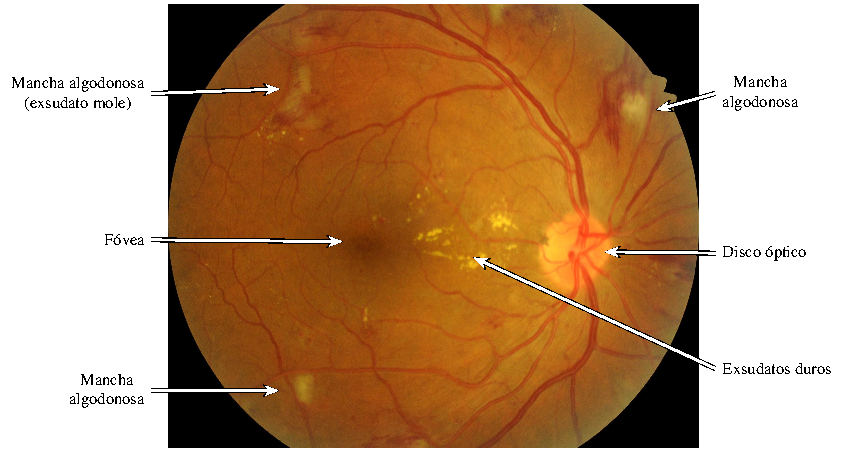
\includegraphics[width=14cm]{figuras/fig-idrid}
	}{
		\Fonte{adaptada de \citeonline{porwal2018idrid}, imagem IDRiD\_22 da base IDRiD (licença \textit{Creative Commons Attribution}), com indicações feitas pelo autor.}
	}
\end{figure}

\subsection{Escala de gravidade da retinopatia diabética}
\label{sec:escala-icdr}

Para padronizar o diagnóstico, \citeonline{wilkinson2003icdr} propuseram a escala internacional de gravidade da retinopatia diabética, conhecida como ICDR (\textit{International Clinical Diabetic Retinopathy}). A escala tem cinco níveis, que vão da ausência de retinopatia até a forma proliferativa, e é a mesma usada como rótulo em bases públicas de classificação, como a do desafio APTOS 2019, organizado pela \textit{Asia Pacific Tele-Ophthalmology Society} \cite{aptos2019}. Os níveis estão apresentados na Tabela~\ref{tab:icdr}.

\begin{table}[!t]
	\caption{\label{tab:icdr} Escala internacional de gravidade da retinopatia diabética (ICDR)}%
	\IBGEtab{}{%
		\begin{tabular}{>{\centering\arraybackslash}p{1.2cm} >{\raggedright\arraybackslash}p{4.2cm} >{\raggedright\arraybackslash}p{9.0cm}}
			\toprule
			Grau & Nível de gravidade & Achados na fundoscopia \\
			\midrule
			0 & Sem retinopatia aparente & Nenhuma alteração \\
			1 & RDNP leve & Apenas microaneurismas \\
			2 & RDNP moderada & Mais do que apenas microaneurismas, mas menos do que a RDNP grave \\
			3 & RDNP grave & Sem sinais de RDP e com qualquer um dos achados: mais de 20 hemorragias intrarretinianas em cada um dos quatro quadrantes; ensalsichamento venoso definido em dois ou mais quadrantes; anormalidades microvasculares intrarretinianas proeminentes em um ou mais quadrantes \\
			4 & RDP & Neovascularização e/ou hemorragia vítrea ou pré-retiniana \\
			\bottomrule
		\end{tabular}%
	}{%
		\Fonte{adaptada de \citeonline{wilkinson2003icdr}.}%
	}
\end{table}

O edema macular é avaliado em uma escala separada, como ausente ou presente e, quando presente, como leve, moderado ou grave, conforme a distância entre o espessamento ou os exsudatos duros e o centro da mácula \cite{wilkinson2003icdr}. Em programas de rastreamento, os graus são agrupados no problema binário de RD referenciável, que reúne os casos de RDNP moderada ou pior e/ou com edema macular, que precisam ser encaminhados a um oftalmologista \cite{gulshan2016}. Como a fotografia não mostra a espessura da retina, \citeonline{krause2018grader} consideraram como edema macular referenciável a presença de exsudatos duros a até um diâmetro de disco do centro da fóvea, uma regra que depende diretamente da localização dos exsudatos.

\section{Pré-processamento de imagens de fundo de olho}
\label{sec:ft-preprocessamento}

As retinografias variam muito em iluminação e contraste, então algumas etapas de pré-processamento ajudam a deixar as imagens mais parecidas entre si. A primeira é o recorte da borda preta ao redor da retina, mantendo apenas o campo de visão. Também é frequente usar só o canal verde, que mostra o maior contraste entre os vasos e o fundo, já que o canal vermelho fica mais saturado e o azul mais escuro \cite{zong2020unet}.

Para melhorar o contraste, a técnica mais usada é a equalização adaptativa de histograma com limite de contraste, o CLAHE (\textit{Contrast Limited Adaptive Histogram Equalization}). A imagem é dividida em pequenas regiões (\textit{tiles}), cada uma é equalizada com o seu próprio histograma e o resultado entre regiões vizinhas é suavizado por interpolação, enquanto o limite de contraste (\textit{clip limit}) corta o histograma em um valor máximo para não amplificar o ruído de áreas homogêneas \cite{pizer1987ahe}. Em imagens coloridas, o CLAHE pode ser aplicado no canal verde ou no canal de luminância (L) do espaço de cor CIELAB, que melhora o contraste sem mexer muito nas cores. Isso é importante aqui, já que os exsudatos duros são amarelados e as manchas algodonosas são mais esbranquiçadas.

O vencedor da competição de RD do Kaggle em 2015 subtraiu de cada imagem uma versão borrada por filtro gaussiano, para destacar detalhes locais e reduzir diferenças de iluminação \cite{graham2015kaggle}. Quando se usam redes pré-treinadas, os pixels também são normalizados com a média e o desvio padrão de cada canal do ImageNet.

A resolução de entrada também importa. Redes pré-treinadas no ImageNet foram pensadas para $224 \times 224$ pixels, mas reduzir uma imagem de $4288 \times 2848$ pixels para esse tamanho torna lesões pequenas praticamente imperceptíveis. \citeonline{sahlsten2019} observaram que resoluções maiores melhoram a gradação da RD, o que leva ao uso de resoluções intermediárias, como 384 ou 512 pixels de lado, como um meio-termo entre o detalhe das lesões e o custo de memória. Na segmentação o problema é ainda maior, o que leva ao uso de recortes em alta resolução (Seção~\ref{sec:seg-lesoes}).

\subsection{Aumento de dados}
\label{sec:aumento-dados}

O aumento de dados (\textit{data augmentation}) gera novas versões das imagens de treino com transformações que não mudam o rótulo, como rotações, espelhamentos, mudanças de escala e alterações de brilho e contraste. Isso reduz o sobreajuste, principalmente em bases pequenas \cite{shorten2019augmentation}. Na segmentação, as transformações geométricas precisam ser aplicadas igualmente na imagem e na máscara. Transformações fortes de cor devem ser usadas com cuidado, porque a cor é uma das pistas que diferenciam exsudatos duros, manchas algodonosas e o disco óptico.

\section{Aprendizado de máquina e aprendizado profundo}
\label{sec:aprendizado}

O aprendizado de máquina reúne métodos em que o computador aprende uma tarefa a partir de exemplos, em vez de seguir regras escritas à mão. No aprendizado supervisionado, que é o caso deste trabalho, cada exemplo de treino tem um rótulo conhecido, como o grau da RD de uma imagem ou a máscara que indica onde estão os exsudatos. O modelo ajusta seus parâmetros para errar o mínimo possível nesses exemplos, e a capacidade de acertar em dados novos é chamada de generalização. O aprendizado profundo (\textit{deep learning}) é uma parte do aprendizado de máquina que usa redes neurais com muitas camadas, capazes de aprender representações dos dados em vários níveis de abstração, diretamente a partir dos pixels \cite{lecun2015deep}.

\subsection{Redes neurais e treinamento}
\label{sec:redes-neurais}

A unidade básica de uma rede neural é o neurônio artificial, que calcula uma soma ponderada das suas entradas e aplica uma função de ativação sobre o resultado, conforme a Equação~\ref{eq:neuronio}:
\begin{equation}
	\label{eq:neuronio}
	y = f\left(\sum_{i=1}^{n} w_i x_i + b\right),
\end{equation}
em que $x_i$ são as entradas, $w_i$ os pesos, $b$ o viés e $f$ a função de ativação. As mais usadas são a unidade linear retificada (ReLU, do inglês \textit{Rectified Linear Unit}), $f(z) = \max(0, z)$, que acelera o treino de redes profundas em relação a funções saturantes como a tangente hiperbólica \cite{krizhevsky2017imagenet}, a sigmoide, usada quando a saída é uma probabilidade entre 0 e 1, e a \textit{softmax}, que gera probabilidades que somam 1 na classificação com várias classes.

Os neurônios são organizados em camadas, e o treinamento consiste em encontrar os pesos que minimizam uma função de perda, que mede a diferença entre a saída da rede e o rótulo esperado. O gradiente da perda em relação a cada peso é calculado pela retropropagação (\textit{backpropagation}), que aplica a regra da cadeia camada por camada, e os pesos são atualizados na direção contrária ao gradiente, em pequenos lotes de exemplos (\textit{mini-batches}), com o tamanho do passo controlado pela taxa de aprendizado \cite{lecun2015deep}.

O Adam é um dos otimizadores mais usados. Ele guarda médias móveis do gradiente e do quadrado do gradiente e, com elas, ajusta o tamanho do passo de cada parâmetro separadamente \cite{kingma2015adam}. O AdamW é uma variação em que o decaimento de pesos (\textit{weight decay}) é aplicado direto sobre os parâmetros, separado da atualização pelo gradiente, o que melhora a regularização em relação ao Adam com penalização L2 \cite{loshchilov2019adamw}.

O sobreajuste (\textit{overfitting}) acontece quando o modelo memoriza os exemplos de treino e passa a errar mais em dados novos. Para reduzir isso, usam-se o decaimento de pesos, o aumento de dados, o \textit{dropout}, que desliga aleatoriamente parte dos neurônios durante o treino \cite{srivastava2014dropout}, e a parada antecipada (\textit{early stopping}), que interrompe o treino quando o desempenho na validação para de melhorar e mantém os pesos da melhor época.

\subsection{Redes neurais convolucionais}
\label{sec:cnn}

As redes neurais convolucionais (CNNs, do inglês \textit{Convolutional Neural Networks}) são redes criadas para dados organizados em grade, como imagens. Em vez de ligar cada pixel a todos os neurônios da camada seguinte, a CNN usa filtros pequenos (\textit{kernels}) que percorrem a imagem e compartilham os mesmos pesos em todas as posições. Com isso, o número de parâmetros se reduz de forma substancial, e a rede consegue detectar o mesmo padrão em qualquer lugar da imagem \cite{lecun2015deep}. A operação de convolução em duas dimensões, para uma entrada $I$ e um filtro $K$ de tamanho $k \times k$, é dada pela Equação~\ref{eq:convolucao}:
\begin{equation}
	\label{eq:convolucao}
	S(i,j) = \sum_{m=0}^{k-1} \sum_{n=0}^{k-1} I(i+m,\, j+n)\, K(m,n).
\end{equation}
A rigor, como o filtro não é invertido, essa equação é uma correlação cruzada, mas é ela que as bibliotecas de aprendizado profundo calculam com o nome de convolução.

O resultado de cada filtro é um mapa de características (\textit{feature map}). O passo (\textit{stride}) define quantos pixels o filtro anda a cada aplicação, e o preenchimento (\textit{padding}) adiciona pixels nas bordas para controlar o tamanho da saída. Depois das convoluções, entra em geral uma camada de \textit{pooling}, que reduz a resolução do mapa. O \textit{max pooling}, por exemplo, mantém o maior valor de cada janela de $2 \times 2$, diminuindo o custo e deixando a rede mais tolerante a pequenos deslocamentos. Ao empilhar camadas, as primeiras aprendem padrões simples, como bordas e cores, e as mais profundas combinam esses padrões em estruturas mais complexas \cite{lecun2015deep}.

\subsection{Transferência de aprendizado e ajuste fino}
\label{sec:transferencia}

Treinar uma rede profunda do zero exige muitas imagens rotuladas, o que é difícil na área médica. Na transferência de aprendizado (\textit{transfer learning}), a rede é inicializada com pesos treinados em uma base grande, normalmente o ImageNet, e depois ajustada para a nova tarefa no ajuste fino (\textit{fine-tuning}), que pode treinar todas as camadas ou congelar as primeiras. \citeonline{raghu2019transfusion} mostraram, em imagens de fundo de olho e radiografias de tórax, que o ganho no desempenho final nem sempre é grande, mas que a convergência fica bem mais rápida. Em bases pequenas como as de lesões, partir de pesos pré-treinados ainda é a escolha mais frequente.

\section{Arquiteturas avaliadas}
\label{sec:ft-arquiteturas}

Este trabalho compara três famílias de redes: modelos tradicionais (VGG16 e ResNet50), modelos leves (MobileNetV3-Large e EfficientNet-B0) e modelos baseados em \textit{Transformers} (ViT-B/16 e Swin-T). As seções a seguir mostram a ideia principal de cada uma, e a Seção~\ref{sec:custo-arquiteturas} compara o número de parâmetros e o custo de cada versão.

\subsection{VGG16}
\label{sec:vgg}

A VGG foi proposta por \citeonline{simonyan2015vgg} com uma ideia simples: usar apenas filtros pequenos, de $3 \times 3$, e aumentar a profundidade. Duas convoluções $3 \times 3$ seguidas cobrem a mesma região que um filtro $5 \times 5$, com menos parâmetros e mais não linearidades, já que são duas ReLU em vez de uma. A VGG16 tem 13 camadas convolucionais em cinco blocos separados por \textit{max pooling} e três camadas totalmente conectadas \cite{simonyan2015vgg}. Por ter uma estrutura simples, ela é bastante usada como codificador em segmentação \cite{iglovikov2018ternausnet}, porém é uma rede pesada, com cerca de 138 milhões de parâmetros \cite{simonyan2015vgg}.

\subsection{ResNet50}
\label{sec:resnet}

Com o aumento da profundidade das redes, foi observado o problema da degradação: a partir de certa profundidade, adicionar camadas fazia o erro de treino aumentar, mesmo sem sobreajuste. \citeonline{he2016resnet} resolveram isso com as redes residuais (ResNets), em que cada bloco aprende apenas uma correção sobre a sua entrada. Em vez de aprender diretamente uma função $\mathcal{H}(\mathbf{x})$, o bloco aprende o resíduo $\mathcal{F}(\mathbf{x}) = \mathcal{H}(\mathbf{x}) - \mathbf{x}$, e a entrada é somada à saída por uma conexão de atalho, conforme a Equação~\ref{eq:residuo} e a Figura~\ref{fig:residual}:
\begin{equation}
	\label{eq:residuo}
	\mathbf{y} = \mathcal{F}(\mathbf{x}, \{W_i\}) + \mathbf{x}.
\end{equation}

\begin{figure}[!t]
	\centering
	\Caption{\label{fig:residual} Diagrama de um bloco residual}
	\UFCfig{}{
		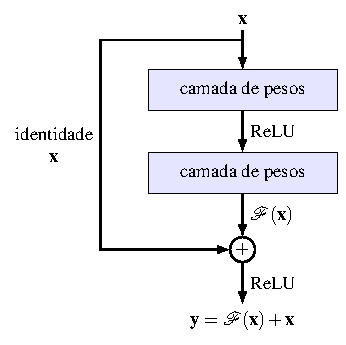
\includegraphics[width=6cm]{figuras/fig-residual}
	}{
		\Fonte{adaptada de \citeonline{he2016resnet}.}
	}
\end{figure}

Esse atalho facilita a passagem do gradiente e permitiu treinar redes com centenas de camadas. Para reduzir o custo computacional, a ResNet50 usa blocos de gargalo (\textit{bottleneck}), com uma convolução $1 \times 1$ que reduz os canais, uma $3 \times 3$ e outra $1 \times 1$ que volta ao número original \cite{he2016resnet}.

\subsection{MobileNetV3}
\label{sec:mobilenet}

As MobileNets foram projetadas para dispositivos móveis. A base de todas é a convolução separável em profundidade (\textit{depthwise separable convolution}), que divide a convolução comum em um filtro $3 \times 3$ aplicado em cada canal separadamente e uma convolução $1 \times 1$ que combina os canais, reduzindo o custo em cerca de oito a nove vezes com pouca perda de acurácia \cite{howard2017mobilenets}. A versão usada neste trabalho é a MobileNetV3-Large, que tem bem menos parâmetros que a VGG16 e a ResNet50 \cite{howard2019mobilenetv3}, sendo pensada para equipamentos com pouca capacidade de processamento. Ela foi encontrada por busca automática de arquitetura a partir dos blocos residuais invertidos da MobileNetV2 \cite{sandler2018mobilenetv2}, com atenção entre canais (\textit{squeeze-and-excitation}) e a ativação \textit{h-swish} \cite{howard2019mobilenetv3}.

\subsection{EfficientNet-B0}
\label{sec:efficientnet}

Aumentar só a profundidade, só a largura ou só a resolução de entrada de uma rede traz ganhos cada vez menores. Partindo dessa observação, \citeonline{tan2019efficientnet} propuseram escalar as três dimensões ao mesmo tempo, de forma balanceada, com um coeficiente $\phi$ e três constantes $\alpha$, $\beta$ e $\gamma$, conforme a Equação~\ref{eq:efficientnet}:
\begin{equation}
	\label{eq:efficientnet}
	d = \alpha^{\phi}, \quad w = \beta^{\phi}, \quad r = \gamma^{\phi}, \quad \text{com } \alpha \cdot \beta^2 \cdot \gamma^2 \approx 2 \text{ e } \alpha, \beta, \gamma \geq 1,
\end{equation}
em que $d$, $w$ e $r$ multiplicam a profundidade, a largura e a resolução da rede base. Essa rede base é a EfficientNet-B0, a versão usada aqui, que foi encontrada por busca de arquitetura e é formada pelos blocos MBConv da MobileNetV2 com atenção entre canais. As versões B1 a B7 saem dela aumentando $\phi$ \cite{tan2019efficientnet}.

\subsection{Transformers e Vision Transformer}
\label{sec:vit}

Os \textit{Transformers} foram criados para tarefas de linguagem natural e se baseiam no mecanismo de autoatenção (\textit{self-attention}), em que cada elemento de uma sequência é atualizado com base em todos os outros \cite{vaswani2017attention}. Cada elemento gera três vetores, chamados de consulta ($Q$), chave ($K$) e valor ($V$), e a atenção é calculada pela Equação~\ref{eq:atencao}:
\begin{equation}
	\label{eq:atencao}
	\text{Attention}(Q, K, V) = \text{softmax}\left(\frac{QK^{T}}{\sqrt{d_k}}\right) V,
\end{equation}
em que $d_k$ é a dimensão das chaves. Na atenção multi-cabeça, várias atenções desse tipo são calculadas em paralelo e os resultados são concatenados, o que permite que o modelo olhe para relações diferentes ao mesmo tempo \cite{vaswani2017attention}.

O Vision Transformer (ViT) levou essa ideia para imagens. A imagem é dividida em pequenos pedaços (\textit{patches}) de $16 \times 16$ pixels, e cada pedaço é transformado em um vetor por uma projeção linear. A esses vetores, chamados de \textit{tokens}, são somados \textit{embeddings} de posição, e um \textit{token} extra de classe (CLS) é colocado no início da sequência. A sequência passa por $L$ blocos do codificador \textit{Transformer}, cada um com autoatenção multi-cabeça e um perceptron multicamadas (MLP, do inglês \textit{Multilayer Perceptron}), e a saída do \textit{token} de classe vai para uma cabeça MLP que dá a classe \cite{dosovitskiy2021vit}, como mostra a Figura~\ref{fig:vit}. Uma imagem de $224 \times 224$ pixels vira, assim, uma sequência de 196 \textit{tokens}. A versão usada aqui é a ViT-B/16, com 12 blocos.

\begin{figure}[!t]
	\centering
	\Caption{\label{fig:vit} Diagrama simplificado do Vision Transformer}
	\UFCfig{}{
		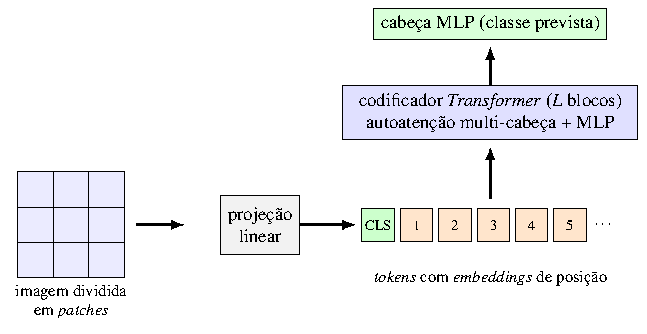
\includegraphics[width=12cm]{figuras/fig-vit}
	}{
		\Fonte{adaptada de \citeonline{dosovitskiy2021vit}.}
	}
\end{figure}

Diferente das CNNs, o ViT não traz embutidas as noções de localidade e de invariância à translação, e por isso, treinado só em bases de tamanho médio, fica abaixo de ResNets de tamanho parecido, melhorando muito com pré-treino em bases maiores \cite{dosovitskiy2021vit}. Em imagens médicas, \citeonline{matsoukas2021cnnvit} observaram que, com pré-treino no ImageNet, os \textit{Transformers} chegam a um desempenho comparável ao das CNNs.

\subsection{Swin Transformer}
\label{sec:swin}

No ViT, cada \textit{token} presta atenção em todos os outros, e o custo cresce com o quadrado do número de \textit{tokens}. Em imagens de alta resolução, esse custo fica alto. Ele também trabalha com uma única escala, o que não combina bem com a segmentação. O Swin Transformer, de \citeonline{liu2021swin}, trata essas duas limitações. A autoatenção é calculada só dentro de janelas locais e, de um bloco para o outro, as janelas são deslocadas (\textit{shifted windows}), para que janelas vizinhas troquem informação. Com isso, o custo passa a crescer de forma linear com o tamanho da imagem. O Swin também é hierárquico: ao longo de quatro estágios, a fusão de \textit{patches} (\textit{patch merging}) junta \textit{tokens} vizinhos e reduz a resolução, gerando mapas em várias escalas, como em uma CNN \cite{liu2021swin}. A versão usada aqui é a menor delas, a Swin-T.

\subsection{Custo das arquiteturas}
\label{sec:custo-arquiteturas}

A Tabela~\ref{tab:arquiteturas} reúne o número de parâmetros e o custo de cada versão para uma imagem de $224 \times 224$ pixels, segundo os artigos originais ou, quando eles não informam, segundo trabalhos posteriores (ver notas da tabela). Parte dos artigos chama esse custo de FLOPs (operações de ponto flutuante, do inglês \textit{Floating Point Operations}), mas \citeonline{he2016resnet}, \citeonline{howard2017mobilenets} e \citeonline{howard2019mobilenetv3} contam explicitamente multiplicações-somas (MACs, do inglês \textit{Multiply-Accumulate operations}), e uma multiplicação-soma equivale a cerca de duas operações. Para não misturar convenções, o custo das redes deste trabalho será medido sempre em MACs e com a mesma ferramenta.

\begin{table}[H]
	\caption{\label{tab:arquiteturas} Parâmetros e custo das arquiteturas comparadas}%
	\IBGEtab{}{%
		\begin{tabular}{llcc}
			\toprule
			Família & Versão & Parâmetros (milhões) & \begin{tabular}[b]{@{}c@{}}Custo de referência a $224 \times 224$\\(GMACs ou GFLOPs, conforme a fonte)\end{tabular} \\
			\midrule
			Tradicional & VGG16 & 138 & 15,3\textsuperscript{b} \\
			Tradicional & ResNet50 & 26\textsuperscript{c} & 3,8 \\
			Leve & MobileNetV3-Large & 5,4 & 0,22 \\
			Leve & EfficientNet-B0 & 5,3 & 0,39 \\
			\textit{Transformer} & ViT-B/16 & 86 & 17,5\textsuperscript{a} \\
			\textit{Transformer} & Swin-T & 29 & 4,5 \\
			\bottomrule
		\end{tabular}%
	}{%
		\Fonte{elaborada pelo autor com dados de \citeonline{simonyan2015vgg}, \citeonline{he2016resnet}, \citeonline{howard2017mobilenets}, \citeonline{howard2019mobilenetv3}, \citeonline{tan2019efficientnet}, \citeonline{dosovitskiy2021vit} e \citeonline{liu2021swin}. \textsuperscript{a}Valor informado por \citeonline{liu2021swin} para o DeiT-B, que tem a mesma arquitetura do ViT-B/16. \textsuperscript{b}Valor informado por \citeonline{howard2017mobilenets}. \textsuperscript{c}Valor informado por \citeonline{tan2019efficientnet}. Nota: valores de referência retirados da literatura, e não medidos neste trabalho. Os custos da VGG16, da ResNet50 e da MobileNetV3-Large são informados pelas fontes como multiplicações-somas (GMACs), e os da EfficientNet-B0, do ViT-B/16 e do Swin-T são chamados de FLOPs (GFLOPs) pelas fontes.}%
	}
\end{table}

\section{Segmentação semântica}
\label{sec:segmentacao}

Na segmentação semântica, cada pixel da imagem recebe uma classe, o que gera uma máscara do mesmo tamanho da imagem. Neste trabalho, a tarefa é indicar quais pixels pertencem a exsudatos duros (EX, do inglês \textit{hard exudates}) e quais pertencem a exsudatos moles (SE, do inglês \textit{soft exudates}). Como as duas lesões são avaliadas separadamente e as máscaras do IDRiD são fornecidas uma para cada lesão \cite{porwal2018idrid}, a rede terá um canal de saída para cada uma, cada canal com uma função sigmoide, que dá a probabilidade de o pixel pertencer àquela lesão.

\subsection{Redes totalmente convolucionais e U-Net}
\label{sec:unet}

As redes totalmente convolucionais (FCNs, do inglês \textit{Fully Convolutional Networks}) foram propostas por \citeonline{long2015fcn}, que trocaram as camadas totalmente conectadas das redes de classificação por convoluções e acrescentaram camadas de aumento de resolução (\textit{upsampling}), de forma que a rede devolve uma predição para cada pixel, combinando mapas profundos, com mais informação semântica, e mapas rasos, com mais detalhes.

A U-Net, proposta por \citeonline{ronneberger2015unet} para imagens biomédicas, organiza essa ideia em forma de U. O codificador aplica convoluções e \textit{pooling} para extrair características e reduzir a resolução, e o decodificador aumenta a resolução aos poucos, concatenando em cada nível os mapas do codificador de mesma resolução por conexões de salto (\textit{skip connections}), o que ajuda a recuperar a localização das estruturas. Os autores mostraram que ela consegue bons resultados com poucas imagens anotadas, com bastante aumento de dados \cite{ronneberger2015unet}, o que é importante para lesões, em que as bases têm poucas dezenas ou centenas de imagens. A estrutura usada neste trabalho, com um codificador pré-treinado, está ilustrada na Figura~\ref{fig:unet}.

\begin{figure}[H]
	\centering
	\Caption{\label{fig:unet} Diagrama de uma U-Net com codificador pré-treinado}
	\UFCfig{}{
		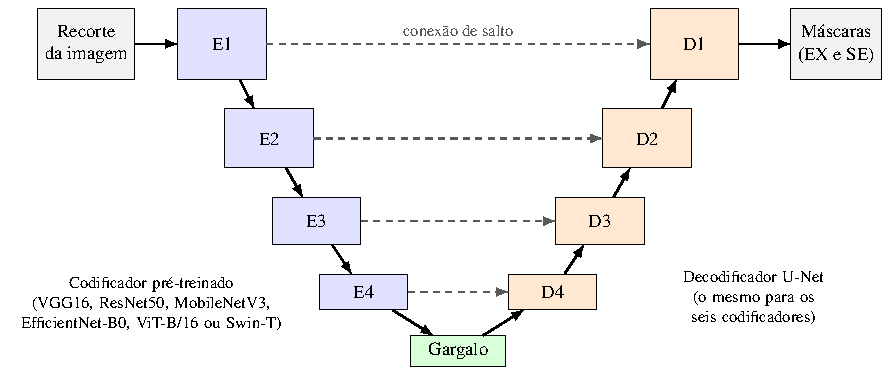
\includegraphics[width=14cm]{figuras/fig-unet}
	}{
		\Fonte{elaborada pelo autor com base em \citeonline{ronneberger2015unet}.}
	}
\end{figure}

\subsection{U-Net com codificadores pré-treinados}
\label{sec:unet-variantes}

\citeonline{iglovikov2018ternausnet} mostraram que trocar o codificador original da U-Net por uma rede de classificação pré-treinada no ImageNet, no caso uma VGG11, melhora a segmentação. Com as CNNs, a troca é direta: os mapas de cada estágio do codificador, em resoluções cada vez menores, vão para as conexões de salto do decodificador. Assim, de um modelo para outro só muda o codificador, e o decodificador continua o mesmo, o que deixa a comparação entre as redes mais controlada.

O Swin-T também se encaixa sem grandes mudanças, porque os seus quatro estágios já geram mapas em 1/4, 1/8, 1/16 e 1/32 da resolução da entrada, como os de uma CNN \cite{liu2021swin}. O ViT é o caso mais difícil, já que todos os seus \textit{tokens} ficam em uma única resolução, de 1/16 da imagem. A UNETR resolve isso extraindo a saída de quatro blocos intermediários do \textit{Transformer} (o 3, o 6, o 9 e o 12), remontando cada sequência de \textit{tokens} como um mapa e reamostrando esses mapas para resoluções diferentes, que então entram nas conexões de salto de um decodificador convolucional \cite{hatamizadeh2022unetr}. A UNETR foi proposta para volumes 3D, mas a mesma ideia pode ser usada em 2D, o que permite ligar um ViT a um decodificador U-Net igual ao usado com as CNNs.

Outras redes já mostraram que \textit{Transformers} funcionam bem como codificadores em U, como a TransUNet \cite{chen2021transunet} e a Swin-Unet \cite{cao2023swinunet}. Cada uma tem o seu próprio decodificador, e o codificador da TransUNet é híbrido, com uma ResNet-50 antes do ViT \cite{chen2021transunet}.

O nome W-Net também aparece na literatura, mas para duas propostas diferentes: duas U-Nets em sequência para segmentação não supervisionada \cite{xia2017wnet} e duas U-Nets muito pequenas em cascata para segmentar vasos da retina \cite{galdran2022wnet}. Nenhuma das duas foi pensada para receber codificadores pré-treinados intercambiáveis.

\subsection{Segmentação de lesões pequenas}
\label{sec:seg-lesoes}

A segmentação de exsudatos tem duas dificuldades principais: o desbalanceamento, já que as lesões ocupam uma fração muito pequena dos pixels, e o tamanho das lesões, muitas com poucos pixels de diâmetro mesmo na resolução original. Por isso, vários trabalhos com o IDRiD treinam com recortes (\textit{patches}) da imagem na resolução original. \citeonline{zong2020unet}, por exemplo, tiraram os recortes das imagens originais com a ajuda de superpixels.

Os recortes podem ser, por exemplo, de $512 \times 512$ pixels, dando preferência a recortes com lesões. Na inferência, a imagem inteira é percorrida por uma janela deslizante (\textit{sliding window}) do mesmo tamanho usado no treino, com sobreposição entre janelas vizinhas, e as predições das regiões sobrepostas são combinadas, como no nnU-Net, em que a sobreposição é de metade do recorte \cite{isensee2021nnunet}. Dessa forma, a imagem inteira não precisa caber de uma vez na memória da unidade de processamento gráfico (GPU, do inglês \textit{Graphics Processing Unit}).

\section{Funções de perda}
\label{sec:perdas}

A função de perda define o que a rede tenta minimizar durante o treino. Na classificação com $C$ classes, a perda mais usada é a entropia cruzada (\textit{cross-entropy}), dada pela Equação~\ref{eq:ce}:
\begin{equation}
	\label{eq:ce}
	\mathcal{L}_{CE} = -\sum_{c=1}^{C} y_c \log(p_c),
\end{equation}
em que $y_c$ vale 1 para a classe correta e 0 para as demais, e $p_c$ é a probabilidade prevista para a classe $c$. Na segmentação, com um canal sigmoide por lesão, usa-se a versão binária dessa perda (BCE, do inglês \textit{Binary Cross-Entropy}), calculada pixel a pixel. Na classificação da RD, como os graus são desbalanceados, cada termo pode ser multiplicado por um peso $w_c$, maior para as classes raras.

Os graus da RD também são ordenados, e errar o grau 4 por 0 é bem pior do que errar por 3. A entropia cruzada não considera essa ordem, então há duas alternativas: tratar o grau como um valor contínuo, com regressão, e depois arredondar por limiares, ou usar uma perda que leve a ordem em conta, como a baseada no kappa ponderado \cite{delatorre2018kappa}. A perda focal (\textit{focal loss}) é outra variação da entropia cruzada, que reduz o peso dos exemplos que a rede já acerta com alta confiança e concentra o treino nos exemplos difíceis \cite{lin2017focal}.

Na segmentação, outra perda muito usada é a \textit{Dice loss}, baseada no coeficiente de Dice, que mede a sobreposição entre a predição e a máscara de referência \cite{milletari2016vnet}. Uma das formas de escrevê-la é a Equação~\ref{eq:dice-loss}:
\begin{equation}
	\label{eq:dice-loss}
	\mathcal{L}_{Dice} = 1 - \frac{2\sum_{i} p_i g_i + \epsilon}{\sum_{i} p_i^2 + \sum_{i} g_i^2 + \epsilon},
\end{equation}
em que $p_i$ é a probabilidade prevista para o pixel $i$, $g_i$ é o seu rótulo (0 ou 1) e $\epsilon$ é uma constante pequena que evita a divisão por zero em recortes sem lesão. Por considerar a sobreposição da lesão como um todo, é menos afetada pela grande quantidade de fundo. Na comparação de \citeonline{ma2021loss}, as perdas compostas, que somam a entropia cruzada e a \textit{Dice loss}, foram as mais estáveis entre diferentes tarefas de segmentação médica.

\section{Validação de modelos}
\label{sec:validacao}

Para saber se um modelo generaliza, ele precisa ser avaliado em dados que não foram usados no treino. Na divisão \textit{hold-out}, a base é separada em treino, validação e teste: a validação serve para escolher hiperparâmetros e decidir quando parar o treino, e o teste é usado só uma vez, no final. Com bases pequenas, porém, o resultado de uma única divisão depende muito de quais imagens caíram em cada parte \cite{varoquaux2018cv}.

Na validação cruzada \textit{k-fold}, a base de desenvolvimento é dividida em $k$ partes (\textit{folds}) e, em cada rodada, uma parte fica separada para avaliação e as outras são usadas no treino. O resultado é a média e o desvio padrão das rodadas. Se o treino usa parada antecipada, ela não pode olhar para o \textit{fold} de avaliação, e por isso uma pequena parte dos \textit{folds} de treino é separada como validação interna. Na versão estratificada, cada parte mantém a proporção de classes, e a versão repetida executa o \textit{k-fold} várias vezes com divisões diferentes \cite{varoquaux2018cv}.

Também é preciso evitar o vazamento de dados (\textit{data leakage}). Ele acontece quando alguma informação do conjunto de avaliação acaba entrando no treino, por exemplo quando imagens do mesmo paciente, como os dois olhos, caem em partes diferentes da divisão, ou quando há imagens duplicadas \cite{kapoor2023leakage}. A solução é a validação cruzada agrupada por paciente (\textit{group k-fold}), em que todas as imagens de um paciente ficam na mesma parte. Escolher hiperparâmetros olhando para o conjunto de teste também é vazamento e deixa a estimativa de desempenho otimista \cite{varma2006bias,cawley2010overfitting}, então a divisão usada na busca não pode ter imagens do teste oficial do IDRiD.

A busca de hiperparâmetros pode ser feita em grade (\textit{grid search}), testando todas as combinações de uma lista de valores, ou de forma aleatória (\textit{random search}), que é mais eficiente quando poucos hiperparâmetros influenciam muito o resultado \cite{bergstra2012random}. Como treinar várias redes profundas é caro, a busca pode ser feita uma vez, em uma divisão de treino e validação, e a validação cruzada rodada só com a melhor configuração de cada arquitetura. Por fim, a validação externa avalia o modelo final em uma base diferente, com outras câmeras e populações, sem nenhum ajuste nela.

\section{Métricas de avaliação}
\label{sec:metricas}

\subsection{Matriz de confusão e métricas derivadas}
\label{sec:matriz-confusao}

Em um problema binário, as predições de um modelo podem ser resumidas na matriz de confusão, apresentada na Tabela~\ref{tab:matriz-confusao}. Os verdadeiros positivos (VP) e verdadeiros negativos (VN) são os acertos, enquanto os falsos positivos (FP) e falsos negativos (FN) são os erros. Na segmentação, a mesma contagem é feita pixel a pixel, considerando a lesão como classe positiva.

\begin{table}[H]
	\caption{\label{tab:matriz-confusao} Matriz de confusão para um problema binário}%
	\IBGEtab{}{%
		\begin{tabular}{lcc}
			\toprule
			& Referência positiva & Referência negativa \\
			\midrule
			Predição positiva & VP & FP \\
			Predição negativa & FN & VN \\
			\bottomrule
		\end{tabular}%
	}{%
		\Fonte{elaborada pelo autor.}%
	}
\end{table}

A partir da matriz, são definidas a acurácia, a precisão, a sensibilidade (ou revocação), a especificidade e o F1-\textit{score}, conforme as Equações~\ref{eq:acuracia} a~\ref{eq:f1}:
\begin{align}
	\text{Acurácia} &= \frac{VP + VN}{VP + VN + FP + FN}, \label{eq:acuracia}\\
	\text{Precisão} &= \frac{VP}{VP + FP}, \\
	\text{Sensibilidade} &= \frac{VP}{VP + FN}, \\
	\text{Especificidade} &= \frac{VN}{VN + FP}, \\
	F_1 &= \frac{2 \cdot \text{Precisão} \cdot \text{Sensibilidade}}{\text{Precisão} + \text{Sensibilidade}}. \label{eq:f1}
\end{align}

No rastreamento da RD, a sensibilidade tem um peso grande, porque um falso negativo é um paciente doente que não foi encaminhado, e por isso o ponto de operação costuma ser escolhido de forma a manter a sensibilidade alta, mesmo com alguma perda de especificidade. Na segmentação, contudo, a acurácia e a especificidade por pixel ficam quase sempre perto de 100\%, já que o fundo domina a imagem, mesmo quando o modelo erra boa parte das lesões \cite{reinke2024pitfalls}. Por isso elas não servem como critério principal.

\subsection{Métricas de segmentação}
\label{sec:ft-metricas-seg}

O coeficiente de Dice (DSC, do inglês \textit{Dice Similarity Coefficient}) e o índice de Jaccard, também chamado de interseção sobre união (IoU, do inglês \textit{Intersection over Union}), medem a sobreposição entre a máscara prevista $P$ e a máscara de referência $G$ \cite{taha2015metrics}, conforme as Equações~\ref{eq:dice} e~\ref{eq:iou}:
\begin{align}
	DSC &= \frac{2\,|P \cap G|}{|P| + |G|} = \frac{2\,VP}{2\,VP + FP + FN}, \label{eq:dice}\\
	IoU &= \frac{|P \cap G|}{|P \cup G|} = \frac{VP}{VP + FP + FN}. \label{eq:iou}
\end{align}
As duas métricas variam entre 0 e 1, estão relacionadas por $DSC = 2\,IoU/(1 + IoU)$ e não usam os verdadeiros negativos, então não são infladas pelo fundo. Quando a imagem não tem a lesão na referência, como acontece em parte das imagens de exsudatos moles, o Dice fica indefinido (0/0) se a predição também estiver vazia e vale zero se houver qualquer falso positivo. Para evitar esse problema, VP, FP e FN podem ser somados em todas as imagens do teste antes de calcular a métrica de cada lesão \cite{reinke2024pitfalls}.

O DSC e o IoU dependem de um limiar para transformar a probabilidade de cada pixel em 0 ou 1, por exemplo 0,5 ou o valor que maximiza o Dice, e esse limiar precisa ser escolhido na validação, e não no teste. Já a área sob a curva de precisão e revocação (AUPR, do inglês \textit{Area Under the Precision-Recall Curve}) não depende de um limiar fixo. Ela é obtida variando o limiar e marcando a precisão e a sensibilidade de cada valor. Em problemas muito desbalanceados, essa curva é mais informativa do que a ROC \cite{saito2015pr}, e a AUPR foi a métrica oficial de segmentação de lesões no desafio do IDRiD \cite{porwal2020idrid}.

\subsection{Métricas de classificação da retinopatia diabética}
\label{sec:ft-metricas-clf}

A curva ROC (\textit{Receiver Operating Characteristic}) mostra a sensibilidade em função de $1 - \text{especificidade}$ para diferentes limiares, e a área sob ela (AUC, do inglês \textit{Area Under the Curve}) vale 0,5 para um classificador aleatório e 1 para um perfeito. Na gradação da RD, ela é mais útil no problema binário de RD referenciável, como em \citeonline{gulshan2016}, junto com a sensibilidade e a especificidade em um ponto de operação escolhido. Um modelo de cinco classes também gera essa AUC: a probabilidade de RD referenciável é a soma das probabilidades previstas para os graus 2, 3 e 4, e é ela que varia com o limiar na curva. Quando a base não traz rótulos de edema macular, a RD referenciável só pode ser definida pelo grau, e os valores deixam de ser diretamente comparáveis aos de estudos que incluem o edema na definição.

Para os cinco graus da escala ICDR, a métrica mais usada é o kappa ponderado quadrático (QWK, do inglês \textit{Quadratic Weighted Kappa}), que foi a métrica da competição APTOS 2019 \cite{aptos2019}. Diferente da acurácia, ele leva em conta a ordem dos graus e pune mais os erros entre graus distantes, como prever grau 0 para um caso de grau 4, do que entre graus vizinhos \cite{cohen1968kappa,fleiss1973kappa}. O QWK é dado pela Equação~\ref{eq:qwk}:
\begin{equation}
	\label{eq:qwk}
	\kappa_w = 1 - \frac{\sum_{i,j} w_{ij}\, O_{ij}}{\sum_{i,j} w_{ij}\, E_{ij}}, \qquad w_{ij} = \frac{(i - j)^2}{(K - 1)^2},
\end{equation}
em que $O_{ij}$ é o número de imagens com grau de referência $i$ e grau previsto $j$, $K$ é o número de graus e $E_{ij}$ é o valor esperado nessa célula se as duas classificações fossem independentes, calculado a partir dos totais de cada linha e de cada coluna e normalizado para ter a mesma soma de $O$. O QWK vale 1 para concordância perfeita, 0 para concordância igual à do acaso e pode ficar negativo quando o modelo é pior que o acaso.

\subsection{Métricas de eficiência}
\label{sec:metricas-eficiencia}

Uma solução CAD para regiões com poucos recursos também precisa ser barata de rodar. \citeonline{canziani2016analysis} mostraram que redes com acurácia parecida podem ter custos de memória, de operações e de tempo de inferência muito diferentes. As medidas mais usadas são o número de parâmetros, que indica o tamanho do modelo, o número de operações (em MACs ou FLOPs) para uma imagem no tamanho de entrada usado, o tempo de inferência por imagem (latência) e o pico de memória durante a inferência. Com essas medidas é possível ver se uma rede mais leve chega a um resultado parecido com o de uma rede maior.

\section{Comparação estatística entre modelos}
\label{sec:estatistica}

Comparar apenas as médias das métricas não basta para dizer que um modelo é melhor que outro, já que parte da diferença pode vir da variação entre as divisões dos dados. As rodadas da validação cruzada também não são independentes, porque os conjuntos de treino se sobrepõem, e os testes que ignoram isso, como o teste \textit{t} pareado comum sobre os \textit{folds}, apontam diferenças significativas com mais frequência do que deveriam \cite{dietterich1998,nadeau2003inference}.

Um dos testes mais usados para comparar dois modelos é o teste dos postos sinalizados de Wilcoxon (\textit{Wilcoxon signed-rank test}) \cite{wilcoxon1945}, recomendado por \citeonline{demsar2006statistical} para esse tipo de comparação e adotado com frequência em trabalhos da área. Ele é um teste não paramétrico para amostras pareadas e, por isso, não exige que as diferenças sigam uma distribuição normal. Para cada rodada $i$, calcula-se a diferença $d_i$ entre as métricas dos dois modelos. As diferenças iguais a zero são descartadas, e as demais são ordenadas pelo valor absoluto $|d_i|$ e recebem postos, do menor para o maior. Em seguida, somam-se os postos das diferenças positivas, obtendo $R^{+}$, e os das diferenças negativas, obtendo $R^{-}$. A estatística do teste é dada pela Equação~\ref{eq:wilcoxon}:
\begin{equation}
	\label{eq:wilcoxon}
	T = \min\{R^{+}, R^{-}\}.
\end{equation}
Quanto menor o valor de $T$, mais as diferenças pendem para um só lado e mais forte é a evidência de que um modelo é melhor que o outro. Com poucas rodadas, o valor-\textit{p} pode ser calculado de forma exata, e, com $n$ diferenças, o menor valor-\textit{p} bilateral possível é $2/2^{n}$, cerca de 0,002 para $n = 10$.

Assim como o teste \textit{t} pareado comum, o Wilcoxon trata as rodadas como independentes. Para levar em conta a sobreposição dos conjuntos de treino, \citeonline{nadeau2003inference} propuseram um teste \textit{t} corrigido, que aumenta a variância estimada de acordo com essa sobreposição. A correção depende do número de rodadas e da proporção entre o tamanho do teste e o do treino, e, na validação cruzada repetida, o número de rodadas é o número de \textit{folds} vezes o número de repetições. Os dois testes podem ser usados juntos, já que o Wilcoxon é o mais usado na área e o teste \textit{t} corrigido considera a dependência entre os \textit{folds}. A forma como eles serão combinados neste trabalho está na Seção~\ref{sec:analise-estatistica}.

Para ordenar vários modelos ao mesmo tempo, \citeonline{demsar2006statistical} recomenda o teste de Friedman \cite{friedman1937ranks}, que ordena os $k$ modelos em cada uma das $N$ medidas e compara os postos médios $R_j$, conforme a Equação~\ref{eq:friedman}:
\begin{equation}
	\label{eq:friedman}
	\chi^2_F = \frac{12N}{k(k+1)} \left[ \sum_{j=1}^{k} R_j^2 - \frac{k(k+1)^2}{4} \right].
\end{equation}
Se houver diferença, o pós-teste de Nemenyi considera dois modelos diferentes quando a diferença entre os seus postos médios passa da diferença crítica (CD, do inglês \textit{Critical Difference}), dada pela Equação~\ref{eq:nemenyi}:
\begin{equation}
	\label{eq:nemenyi}
	CD = q_{\alpha} \sqrt{\frac{k(k+1)}{6N}},
\end{equation}
em que $q_{\alpha}$ é um valor tabelado que depende de $k$ e do nível de significância \cite{demsar2006statistical}. Esse teste foi pensado para comparar modelos em várias bases de dados independentes. Quando ele é aplicado aos \textit{folds} de uma mesma base, os \textit{folds} não são independentes, e o resultado deve ser visto como uma ordenação dos modelos, mostrada no diagrama de diferença crítica, e não como prova definitiva.

Nos conjuntos de teste fixos, como o teste oficial do IDRiD e as bases externas, usa-se o \textit{bootstrap} \cite{efron1979bootstrap}. As imagens do teste são sorteadas com reposição muitas vezes (por exemplo, mil) e a métrica é recalculada em cada amostra, gerando um intervalo de confiança de 95\%. Para comparar dois modelos, o sorteio é pareado: as mesmas imagens sorteadas valem para os dois, e o intervalo é calculado para a diferença entre eles. Para a AUC, o teste de DeLong compara as áreas de duas curvas obtidas nas mesmas imagens \cite{delong1988}. Quando vários pares são testados, os valores-\textit{p} são corrigidos pelo método de Holm, que os ordena do menor para o maior, compara o $i$-ésimo com $\alpha/(m - i + 1)$, sendo $m$ o número de comparações, e para no primeiro que não for rejeitado, mantendo os seguintes \cite{holm1979simple}. Além do valor-\textit{p}, também será mostrada a diferença entre os modelos com o seu intervalo, para saber se o ganho é grande ou pequeno.

\section{Sistemas de apoio ao diagnóstico}
\label{sec:cad}

Nos sistemas CAD, o médico usa o resultado de uma análise computacional das imagens como uma segunda opinião \cite{doi2007cad}. A decisão final continua com o profissional, e o sistema ajuda a apontar regiões suspeitas e a agilizar a triagem. Na RD, o uso de aprendizado profundo ganhou força depois que \citeonline{gulshan2016} mostraram que uma CNN detectava a RD referenciável com desempenho próximo ao de oftalmologistas, e em 2018 o IDx-DR se tornou o primeiro sistema autônomo de inteligência artificial autorizado pela agência reguladora dos Estados Unidos (FDA, do inglês \textit{Food and Drug Administration}), para a detecção da RD na atenção primária \cite{abramoff2018pivotal}.

Em um sistema CAD, o profissional precisa entender de onde veio o resultado. Na classificação, isso pode ser feito com mapas de ativação como o Grad-CAM (\textit{Gradient-weighted Class Activation Mapping}), que destacam as regiões da imagem que mais pesaram na decisão da rede \cite{selvaraju2017gradcam}. Na segmentação, a própria máscara já funciona como explicação, porque mostra onde estão as lesões encontradas. Por isso, mostrar a máscara dos exsudatos junto com o grau previsto pode ajudar o profissional a conferir o que o sistema encontrou.

Além de ser exibida ao profissional, a segmentação também pode ser usada na própria decisão do sistema. A forma mais simples é a regra de edema macular vista na Seção~\ref{sec:escala-icdr}: se a máscara tiver exsudatos duros a até um diâmetro de disco do centro da fóvea (para isso, é preciso localizar o centro da fóvea e o disco óptico na imagem), a imagem é marcada como suspeita de edema macular referenciável \cite{krause2018grader}, o que acrescenta uma informação que o classificador de graus, sozinho, não fornece. Uma alternativa mais avançada são os modelos guiados por lesão, em que a segmentação ajuda diretamente a gradação, como no aprendizado colaborativo de \citeonline{zhou2019collaborative} e nos \textit{Transformers} com atenção às lesões de \citeonline{sun2021lesion}. A forma como os dois módulos serão integrados na solução CAD deste trabalho é descrita no Capítulo~\ref{chap:metodologia}.
